\documentclass[fullscreen=true, unicode, bookmarks=false]{beamer}
\usepackage[T2A]{fontenc}
\usepackage[utf8]{inputenc}
\usepackage[english, russian]{babel}
\usepackage{amsmath}
\usepackage{amsmath,amsfonts,amssymb}
\usepackage[export]{adjustbox}
\usepackage{textgreek}
\newtheorem{rustheorem}{Теорема }
\sloppy

\setbeamertemplate{navigation symbols}{}

\usetheme{Madrid}

\usecolortheme{whale}

\usefonttheme{professionalfonts} % default family is serif

\setbeamertemplate{footline}{\hspace*{.5cm}\scriptsize{\insertshorttitle
\hspace*{50pt} \hfill\hspace*{.5cm}}\vspace{5pt}} 

\setbeamercolor{bibliography entry author}{fg=black}

\title[]{ Потеря устойчивости нулевого состояния равновесия одной краевой задачи с линейным отклонением в краевом условии }   
\author[]{{\Large Леонид Ивановский}} 
\date{}
\institute[]
{  }
\titlegraphic{
   \vspace{-1.5cm}
   
\includegraphics[scale = 0.22]{yarsu_logo.jpg}
}

\begin{document}

\begin{frame}
\titlepage
\end{frame} 

\begin{frame}
\frametitle{ Краевая задача с отклонением в краевом условии }
 
\begin{equation}
	\dot u = u'' + \gamma u - u^3,	
\end{equation}

\begin{equation}
	u'(0, t) \, = 0, \qquad u'(1, t) \, = \alpha\,u(x_0, t),
\end{equation}

\bigskip

$$ \alpha, \gamma \in \mathbb{R}, \quad x_0 \in [0, 1). $$

\end{frame}

\begin{frame}
\frametitle{ Линеаризованная краевая задача }
 
\begin{equation}
	\dot u = u'' + \gamma u,	
\end{equation}

\begin{equation}	
	u'(0, t) \, = 0, \qquad u'(1, t) \, = \alpha\,u(x_0, t).
\end{equation}

\end{frame}

\begin{frame}
\frametitle{ Задача на собственные значения }
 
$$ u(x, t) = e^{\lambda t} \, v(x). $$

\bigskip
\pause
 
\begin{equation}
	v'' + (\gamma - \lambda)v = 0,	
\end{equation}

\begin{equation}	
	v'(0) \, = 0, \qquad v'(1) \, = \alpha\,v(x_0).
\end{equation}

\bigskip
\pause

$$ \mu = \sqrt{-\gamma + \lambda}, $$

$$ v(x) = c \, \mbox{ch}  \mu x, \quad c \in \mathbb{R}. $$

\end{frame}

\begin{frame}
\frametitle{ Потеря устойчивости нулевого состояния равновесия }
 
\begin{equation}
	\mu \, \mbox{sh} \mu \, = \, \alpha \mbox{ch} \mu x_0,
\end{equation}

\medskip
\pause

\begin{itemize}

\item { $ \lambda = 0: \; \mu = \sqrt{-\gamma}, $ 
}

$$ \alpha_u = \frac{ \sqrt{-\gamma} \, \mbox{sh} \sqrt{-\gamma} }{ \mbox{ch} \sqrt{-\gamma} x_0 }. $$

\pause
\item { $ \lambda = \pm i \omega: \; \mu = \sqrt{-\gamma + i \omega}, $ 
}

$$ \alpha_c = \frac{ \sqrt{-\gamma + i \omega} \, \mbox{sh} \sqrt{-\gamma + i \omega} }{ \mbox{ch} \sqrt{-\gamma + i \omega} x_0 }. $$

\end{itemize}	

\end{frame}

\begin{frame}
\frametitle{ Схематическая визуализация критической зависимости }

\begin{figure} 
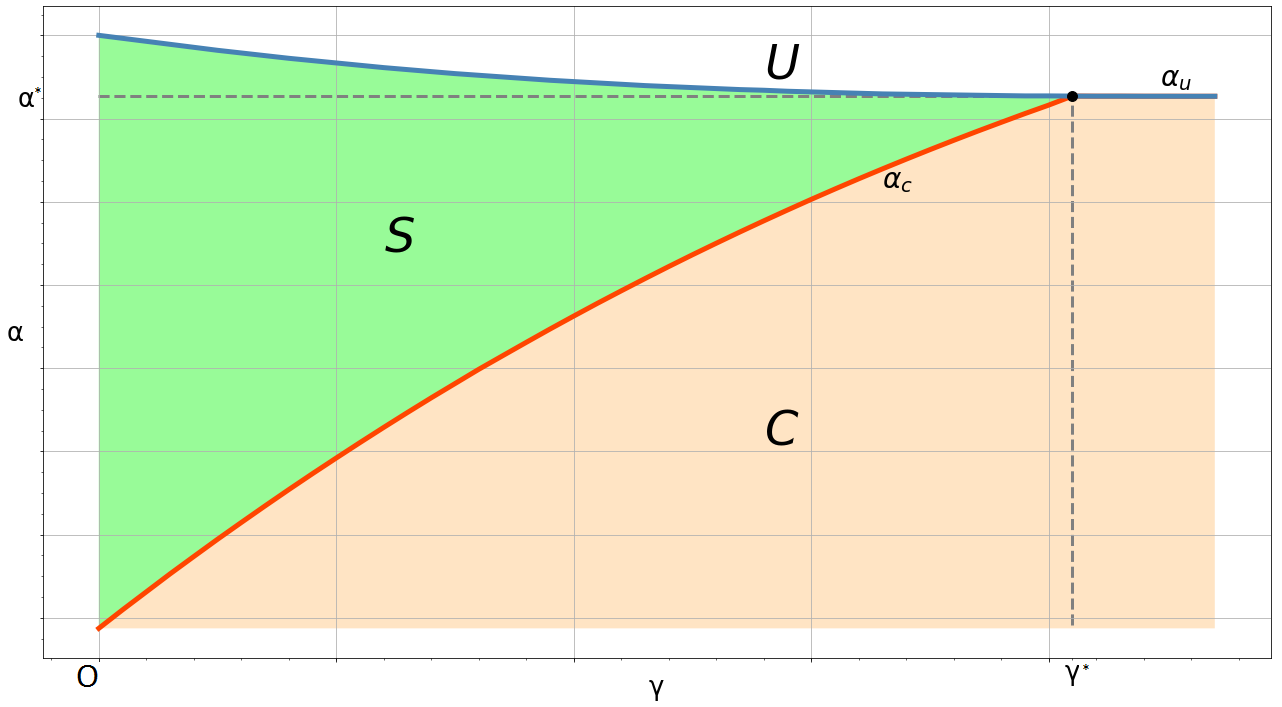
\includegraphics[scale=0.35]{scheme.png}  
\end{figure}

\end{frame}

\begin{frame}
\frametitle{ Численные результаты: $ \alpha_{cr}(\gamma) $ }

\begin{figure} 
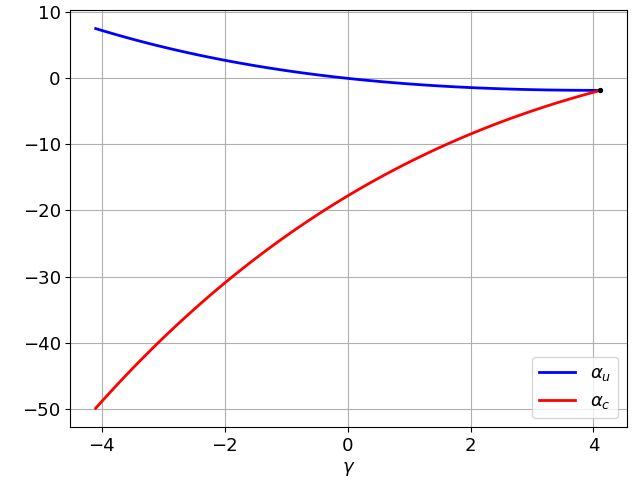
\includegraphics[scale=0.55]{alphas_0.png}  
\end{figure}

$$ x_0 = 0: \quad \gamma_* \approx 4.115 $$

\end{frame}

\begin{frame}
\frametitle{ Численные результаты: $ \alpha_{cr}(\gamma) $ }

\begin{figure} 
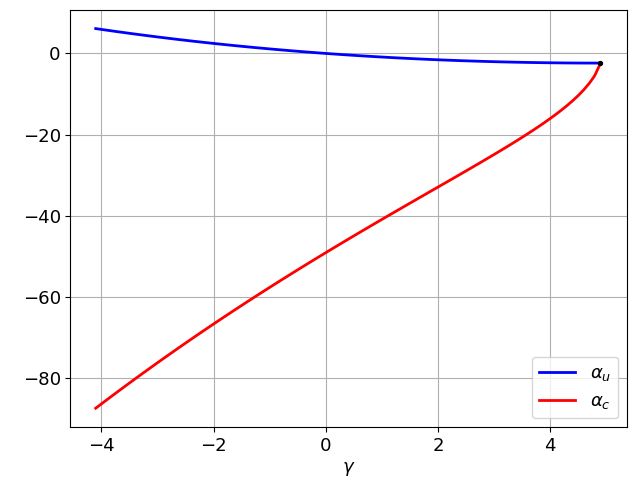
\includegraphics[scale=0.55]{alphas_13.png}  
\end{figure}

$$ x_0 = 0.33: \quad \gamma_* \approx 4.895 $$

\end{frame}

\begin{frame}
\frametitle{ Численные результаты: $ \alpha_{cr}(\gamma) $ }

\begin{figure} 
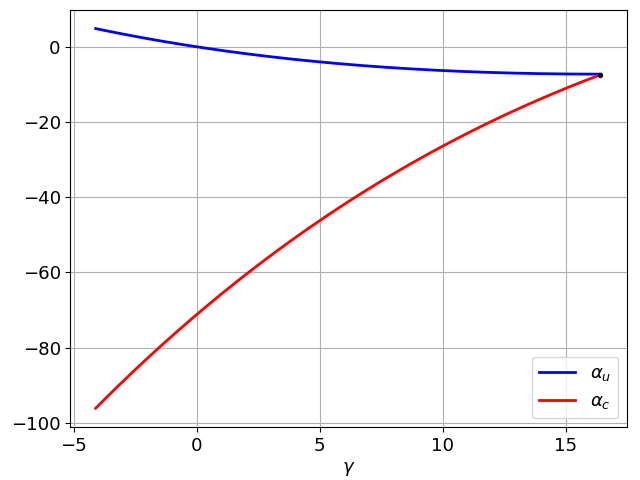
\includegraphics[scale=0.55]{alphas_12.png}  
\end{figure}

$$ x_0 = 0.5: \quad \gamma_* \approx 16.4 $$

\end{frame}

\begin{frame}
\frametitle{ Численные результаты: $ \alpha_{cr}(\gamma) $ }

\begin{figure} 
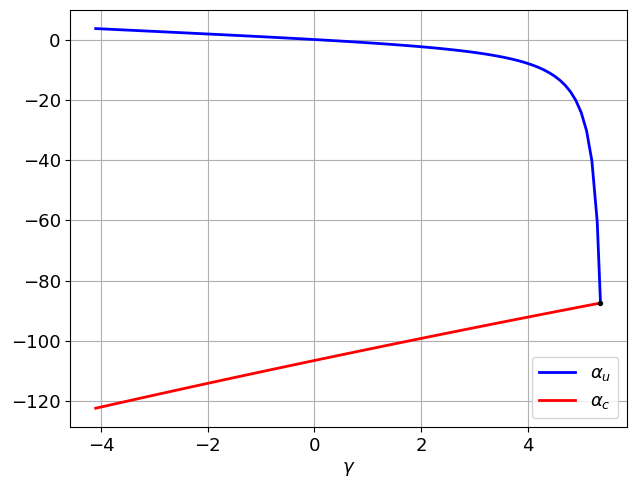
\includegraphics[scale=0.55]{alphas_23.png}  
\end{figure}

$$ x_0 = 0.67: \quad \gamma_* \approx 5.361 $$

\end{frame}

\begin{frame}
\frametitle{ Локальный анализ краевой задачи }

\begin{equation}
	u = \sqrt{\varepsilon}u_0 + \varepsilon u_1 + \varepsilon^{\frac{3}{2}} u_2 + O(\varepsilon^2),
\end{equation}

\bigskip

$$ \varepsilon \ll 1, \quad s = \varepsilon t. $$

\end{frame}

\begin{frame}
\frametitle{ Случай дивергентной потери устойчивости }

\begin{itemize}
\item { $ \lambda = 0: \quad \varepsilon=\alpha-\alpha_u, $
}
\end{itemize}

\bigskip

\begin{equation}
	u_0 = \rho(s) \mbox{ch} \sqrt{-\gamma} x.
\end{equation}

\end{frame}

\begin{frame}
\frametitle{ Случай дивергентной потери устойчивости }

\begin{equation}
	\rho' = \phi_0 \rho + d_0 \rho^3,
\end{equation}

\bigskip
\pause

$$ \phi_0 = \frac{ 2 \mu \mbox{ch} \mu x_0 }{ \mu \mbox{ch} \mu +\mbox{sh} \mu - \alpha_u x_0 \mbox{sh} \mu x_0 }, $$
$$ d_0 = \frac{ -3\gamma \mbox{sh} 3\mu - 12 \mbox{sh} \mu - 12 \mu \mbox{ch} \mu - \alpha_u \mu \mbox{ch} 3\mu x_0 + 12 \alpha_u x_0 \mbox{sh} \mu x_0 }{ 16( \mbox{sh} \mu + \mu \mbox{ch} \mu - \alpha_u x_0 \mbox{sh} \mu x_0 ) }, $$

$$ \mu = \sqrt{-\gamma}. $$

\end{frame}

\begin{frame}
\frametitle{ Численные результаты: $ \phi(\gamma) $ и $ d(\gamma) $ }

\begin{figure} 
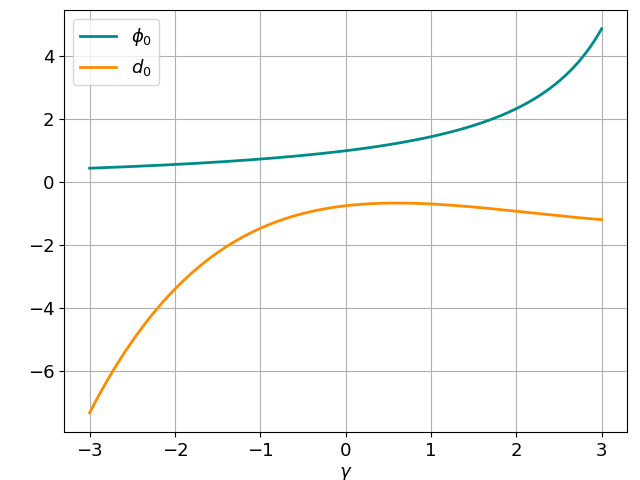
\includegraphics[scale=0.55]{divergent_phi0d0_0.png}  
\end{figure}

$$ x_0 = 0 $$

\end{frame}

\begin{frame}
\frametitle{ Численные результаты: $ d(\gamma) $ }

\begin{figure} 
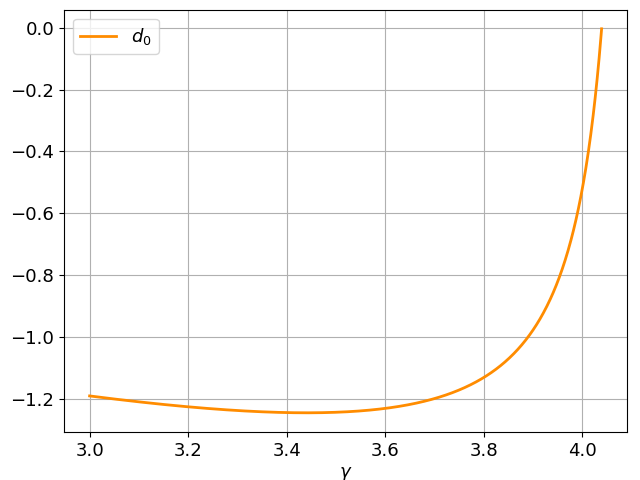
\includegraphics[scale=0.37]{divergent_d0_before_0.png}  
\hfill
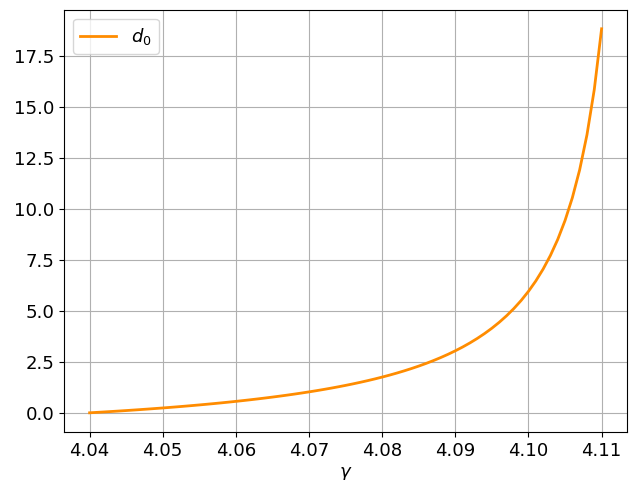
\includegraphics[scale=0.37]{divergent_d0_after_0.png}  
\end{figure}

$$ x_0 = 0: \quad \gamma_l \approx 4.039, \; \gamma_* \approx 4.115 $$

\end{frame}

\begin{frame}
\frametitle{ Численные результаты: $ \phi(\gamma) $ и $ d(\gamma) $ }

\begin{figure} 
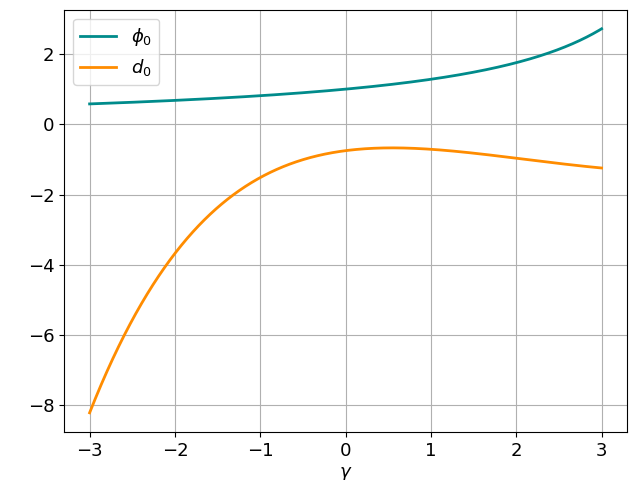
\includegraphics[scale=0.55]{divergent_phi0d0_13.png}  
\end{figure}

$$ x_0 = 0.33 $$

\end{frame}

\begin{frame}
\frametitle{ Численные результаты: $ d(\gamma) $ }

\begin{figure} 
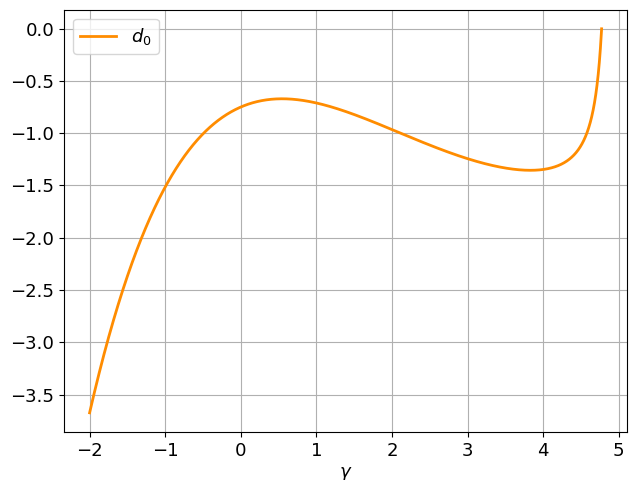
\includegraphics[scale=0.37]{divergent_d0_before_13.png}  
\hfill
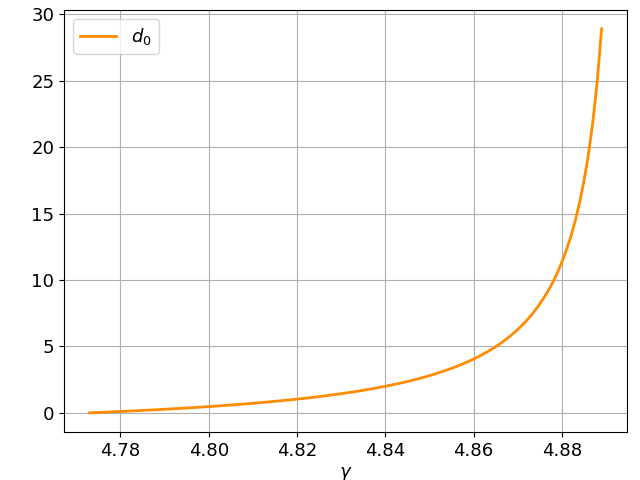
\includegraphics[scale=0.37]{divergent_d0_after_13.png}  
\end{figure}

$$ x_0 = 0.33: \quad \gamma_l \approx 4.773, \; \gamma_* \approx 4.895 $$

\end{frame}

\begin{frame}
\frametitle{ Численные результаты: $ \phi(\gamma) $ и $ d(\gamma) $ }

\begin{figure} 
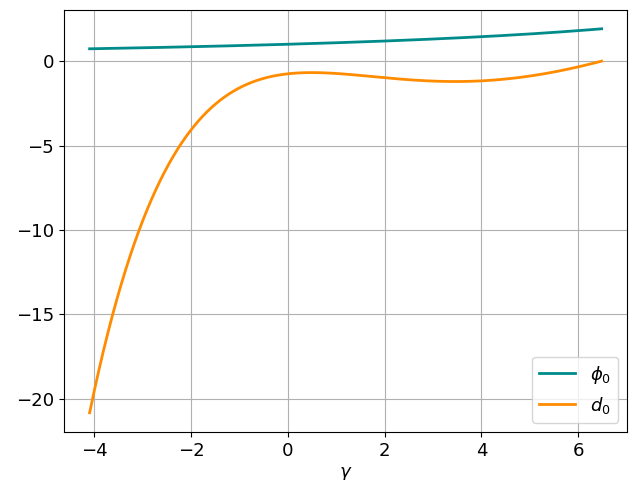
\includegraphics[scale=0.37]{divergent_phi0d0_12_1.png}  
\hfill
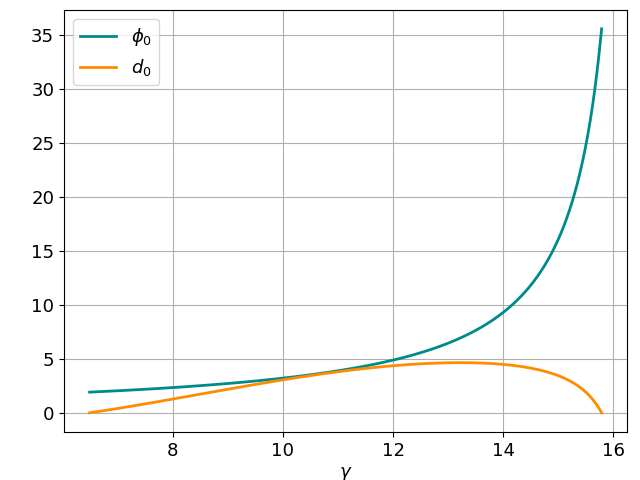
\includegraphics[scale=0.37]{divergent_phi0d0_12_2.png}  
\end{figure}

$$ x_0 = 0.5: \quad \gamma_l \approx 6.485, \; \gamma_{l_*} \approx 15.792, \; \gamma_* \approx 16.4 $$

\end{frame}

\begin{frame}
\frametitle{ Численные результаты: $ \phi(\gamma) $ и $ d(\gamma) $ }

\begin{figure} 
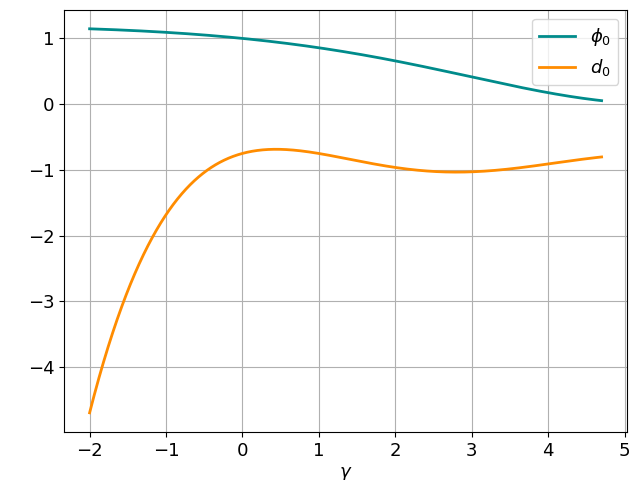
\includegraphics[scale=0.55]{divergent_phi0d0_23.png}  
\end{figure}

$$ x_0 = 0.67: \quad \gamma_* \approx 5.361 $$

\end{frame}

\begin{frame}
\frametitle{ Случай колебательной потери устойчивости }

\begin{itemize}
\item { $ \lambda = \pm i \omega: \quad \varepsilon=\alpha_c-\alpha, $
}
\end{itemize}

\bigskip

\begin{equation}
	u_0 = z(s) e^{i \omega t} \mbox{ch} \mu x + \overline{z(s)} e^{-i \omega t} \overline{\mbox{ch} \mu x}.
\end{equation}

\end{frame}

\begin{frame}
\frametitle{ Случай колебательной потери устойчивости }

\begin{equation}
	z' = \phi_0 z + d_0 z |z|^2,
\end{equation}

$$ \phi_0 = \mbox{Re} \phi, \quad d_0 = \mbox{Re} d, $$

\bigskip
\pause

$$ \phi = \frac{ 2 \mu \mbox{ch} \mu x_0 }{ \mu \mbox{ch} \mu +\mbox{sh} \mu - \alpha_c x_0 \mbox{sh} \mu x_0 }, $$

$$ d = \frac{ 3 \mu ( G(\mu + 2\,\mbox{Re}\mu) + G(\mu + 2i\,\mbox{Im}\mu) + 2G(\overline{\mu}) ) }{ 2 ( \mu \mbox{ch} \mu +\mbox{sh} \mu - \alpha_c x_0 \mbox{sh} \mu x_0 ) }, $$

$$ \mu = \sqrt{-\gamma + i \omega}, $$

$$ G(y) = \frac{ \alpha_c - y\,\mbox{sh} y }{ y^2 + \gamma - i\omega }. $$

\end{frame}

\begin{frame}
\frametitle{ Численные результаты: $ \phi_0(\gamma) $ и $ d_0(\gamma) $ }

\begin{figure} 
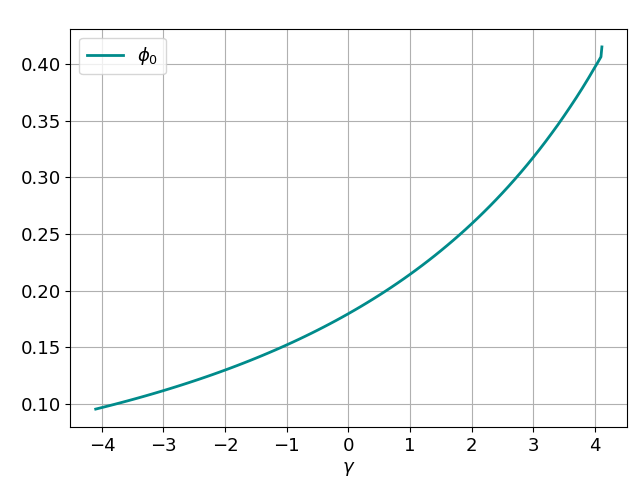
\includegraphics[scale=0.37]{oscillating_phi0_0.png}  
\hfill
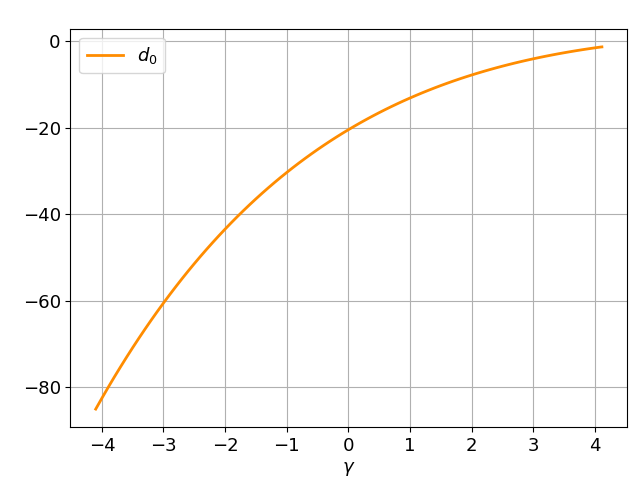
\includegraphics[scale=0.37]{oscillating_d0_0.png}  
\end{figure}

$$ x_0 = 0 $$

\end{frame}

\begin{frame}
\frametitle{ Численные результаты: $ \phi_0(\gamma) $ и $ d_0(\gamma) $ }

\begin{figure} 
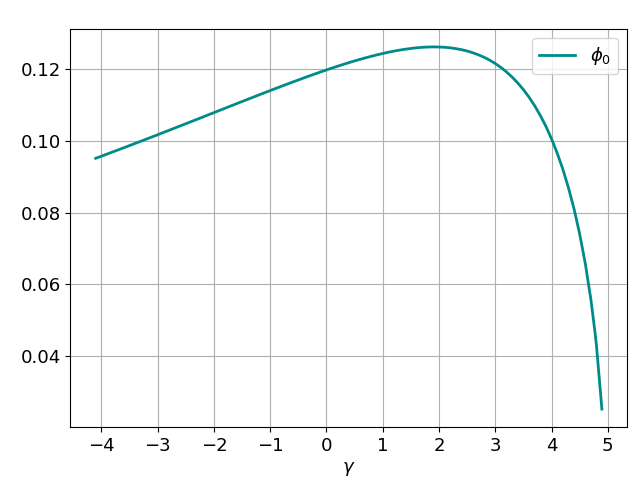
\includegraphics[scale=0.37]{oscillating_phi0_13.png}  
\hfill
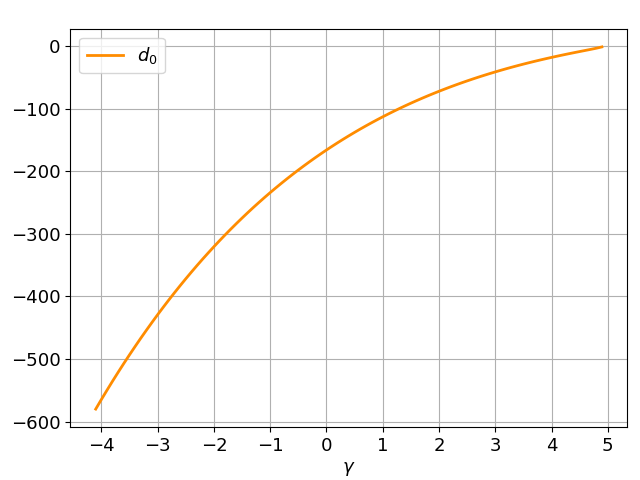
\includegraphics[scale=0.37]{oscillating_d0_13.png}  
\end{figure}

$$ x_0 = 0.33 $$

\end{frame}

\end{document}